\chapter{ストロー飛行機の作成}



\section{翼の加工方法}
\subsection{カッター}
前章で製作した図面を印刷しカッターで切り出す.最初は定規を当てず切っていたが微妙なズレが生じ,飛行距離に差が生じた.そのため定規を当てながら切る事でズレを生じさせないようにした.しかしカッターを用いる欠点としては一機作るために約30~40分かかるため多大な時間がかかる・大量生産が出来ない・ズレが生じるという欠点があったため違う加工方法を模索することにした.次に同じカッターでも図面の線を極限まで細くし,カッターを定規に当てながら加工を行った.結果は以前より格段に加工精度が上昇したが手作業のため直角が出し切れず,ズレが生じてしまった.そのため次にレーザ加工を実践することに決めた.

\subsection{レーザ加工}
次にレーザ加工を用いて加工する事にした.まずCAD上で作成した翼を図面化し,その後dxfファイルに変換することでレーザ加工ファイルを作る.まず加工する前に実験を行い最適な数値の決定を行った.実験の結果を表\ref{tab:experiment}に示す.

\begin{table}[H]
 \begin{center}
   \caption{レーザ実験結果}
   \begin{tabular}[htbp]{|c|c|c|}
    \hline
    スピード(S)&パワー(W)&結果 \\
    \hline
    5.0&20&切れるが少し焦げ臭い\\
    \hline
    6.0&20&焦げないが約1割が切り取りにくい\\
    \hline
    7.0&20&約5割が切れない\\
    \hline
    8.0&20&約7割が切れない\\
    \hline
    5.0&19&焦げ臭さが薄くなった\\
    \hline
    6.0&19&約1.5割が切れない\\
    \hline
    7.0&19&約6割が切れない\\
    \hline
    8.0&19&約8割が切れない\\
    \hline
    5.0&18&加工後ススが出る\\
    \hline
    6.0&18&約2割が切れない\\
    \hline
    7.0&18&約7割が切れない\\
    \hline
    8.0&18&約9割が切れない\\
    \hline
    5.0&17&綺麗な加工断面が得られるが多少ススが出る\\
    \hline
    6.0&17&約3割が切れない\\
    \hline
    7.0&17&約9.5割が切れない\\
    \hline
    8.0&17&ほぼ10割が切れない\\
    \hline
    5.0&16&焦げてる部分がなくススも出ない\\
    \hline
    6.0&16&約3割が切れない\\
    \hline
    7.0&16&ほぼ10割切れない\\
    \hline
    8.0&16&完全に貫通しなくなる\\
    \hline
   \end{tabular}
   \label{tab:experiment}
  \end{center}
\end{table}


以上の結果からS:5.0 P:16が一番最適な数値だと判断した.このことから1mmのケント紙をレーザ加工で製作する場合この数値を用いると綺麗な断面が得られる.がある.レーザ加工の利点としては機械が加工してくれるためズレが生じない・一機約2分で出来る・大量生産が出来るといったメリットがある.しかし欠点としては学校で一機しかレーザ加工機がないため順番待ちになってしまう場合があり予定通りに作業が進まないといった欠点がある.またフォーカスを調整するときオートフォーカスピンを用いるとオートフォーカスピンがケント紙に触れず限界高さを迎えてしまう.そのため自分でフォーカスを合わせるマニュアルピンを用いるため前回とズレが生じる可能性があるため前回と同じ加工精度を出せる保証はないというデメリットがある.

\section{接着方法}
翼とストロー本体を接着する方法としていくつかの方法を用いた.以下に結果を示す.
\begin{table}[H]
 \begin{center}
   \caption{接着方法}
   \begin{tabular}[htbp]{|c|c|}
    \hline
    接着方法&結果 \\
    \hline
    セロハンテープ&強度もよく取り付けが容易・翼が傾く\\
    \hline
    スティックのり&翼が傾かない・接着に時間がかかる・強度が足りない\\
    \hline
    木工用ボンド&接着に時間がかかる・木工用であるため接着するのに適しない\\
    \hline
    スコッチ強力接着剤&翼が傾かずずれない・取り付けが容易・強度が高い\\
    \hline
    \end{tabular}
   \label{tab:experiment}
  \end{center}
\end{table}

以上よりスコッチ強力接着剤を用いる事に決めた.しかし接着した瞬間固まるため微調整が出来ないという欠点がある.
次に翼2枚を接着するための方法を考えた.最初の頃は翼1枚で製作していたが強度がなくすぐヘロヘロになるため強度を上げるために同じ翼2枚を貼り合わせて強度を出すことにした.
まずスコッチ強力接着剤を用いたが先述した通りすぐ固まるため微調整が出来ずピッタリ2枚を貼り合わせる事が出来なかった.次に木工用ボンドを用いて接着をおこなった.木工用ボンドを用いるとムラがなくすぐ固まらないので綺麗に張り合わすことが出来た.しかし木工用ボンドで接着するには注意点があり木工用ボンドを指や刷毛を用いるなどして翼全体にムラなく伸ばさないと固まった時段差が出来てしまい飛行機が真っすぐ飛ばないといった事が起こる.また固まるまで翼の上から重しを載せておかないと木工用ボンドの影響で翼が反ってしまい綺麗な真っすぐした翼が出来ないといった欠点がある.綺麗な翼を図\ref{fig:OK},凸凹な翼を図\ref{fig:NG}に示す.スコッチ強力接着剤を図\ref{fig:sc}に示す.


\begin{figure}[htbp]
  \begin{center}
    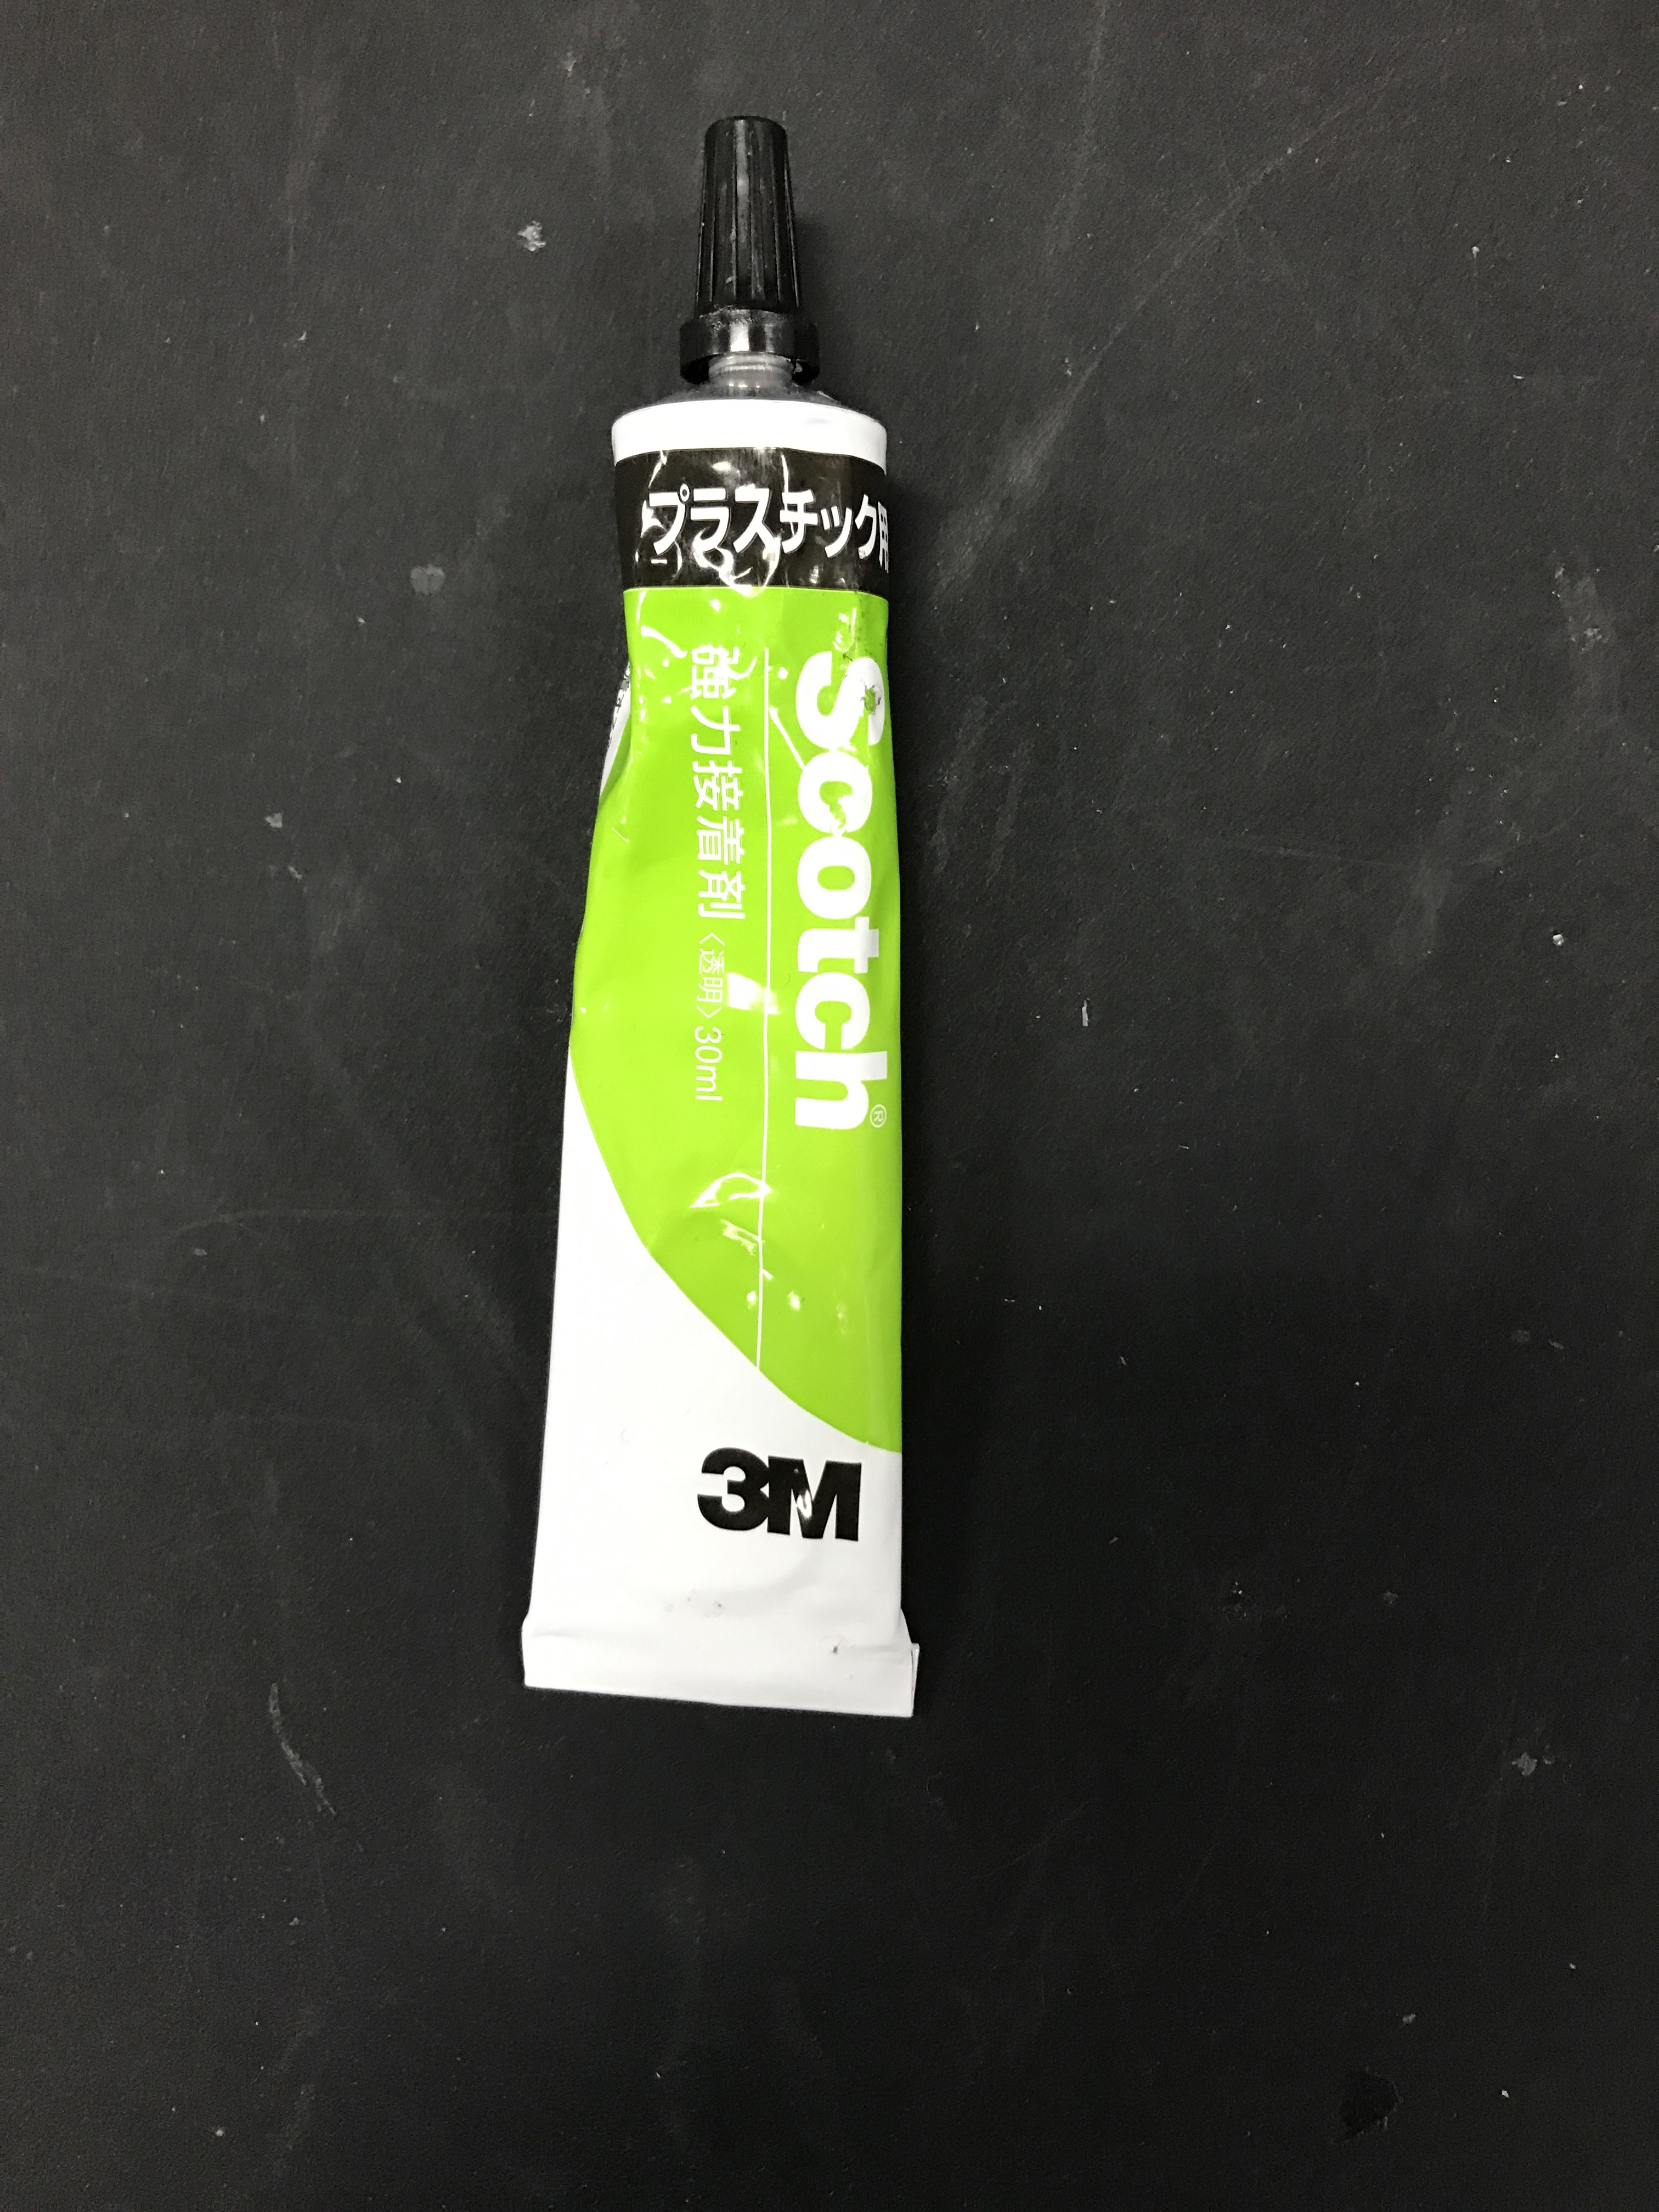
\includegraphics[width=140mm]{sc.JPG}
    \end{center}
  \caption{スコッチ強力接着剤}
 \label{fig:sc}
\end{figure}


\begin{figure}[htbp]
  \begin{center}
    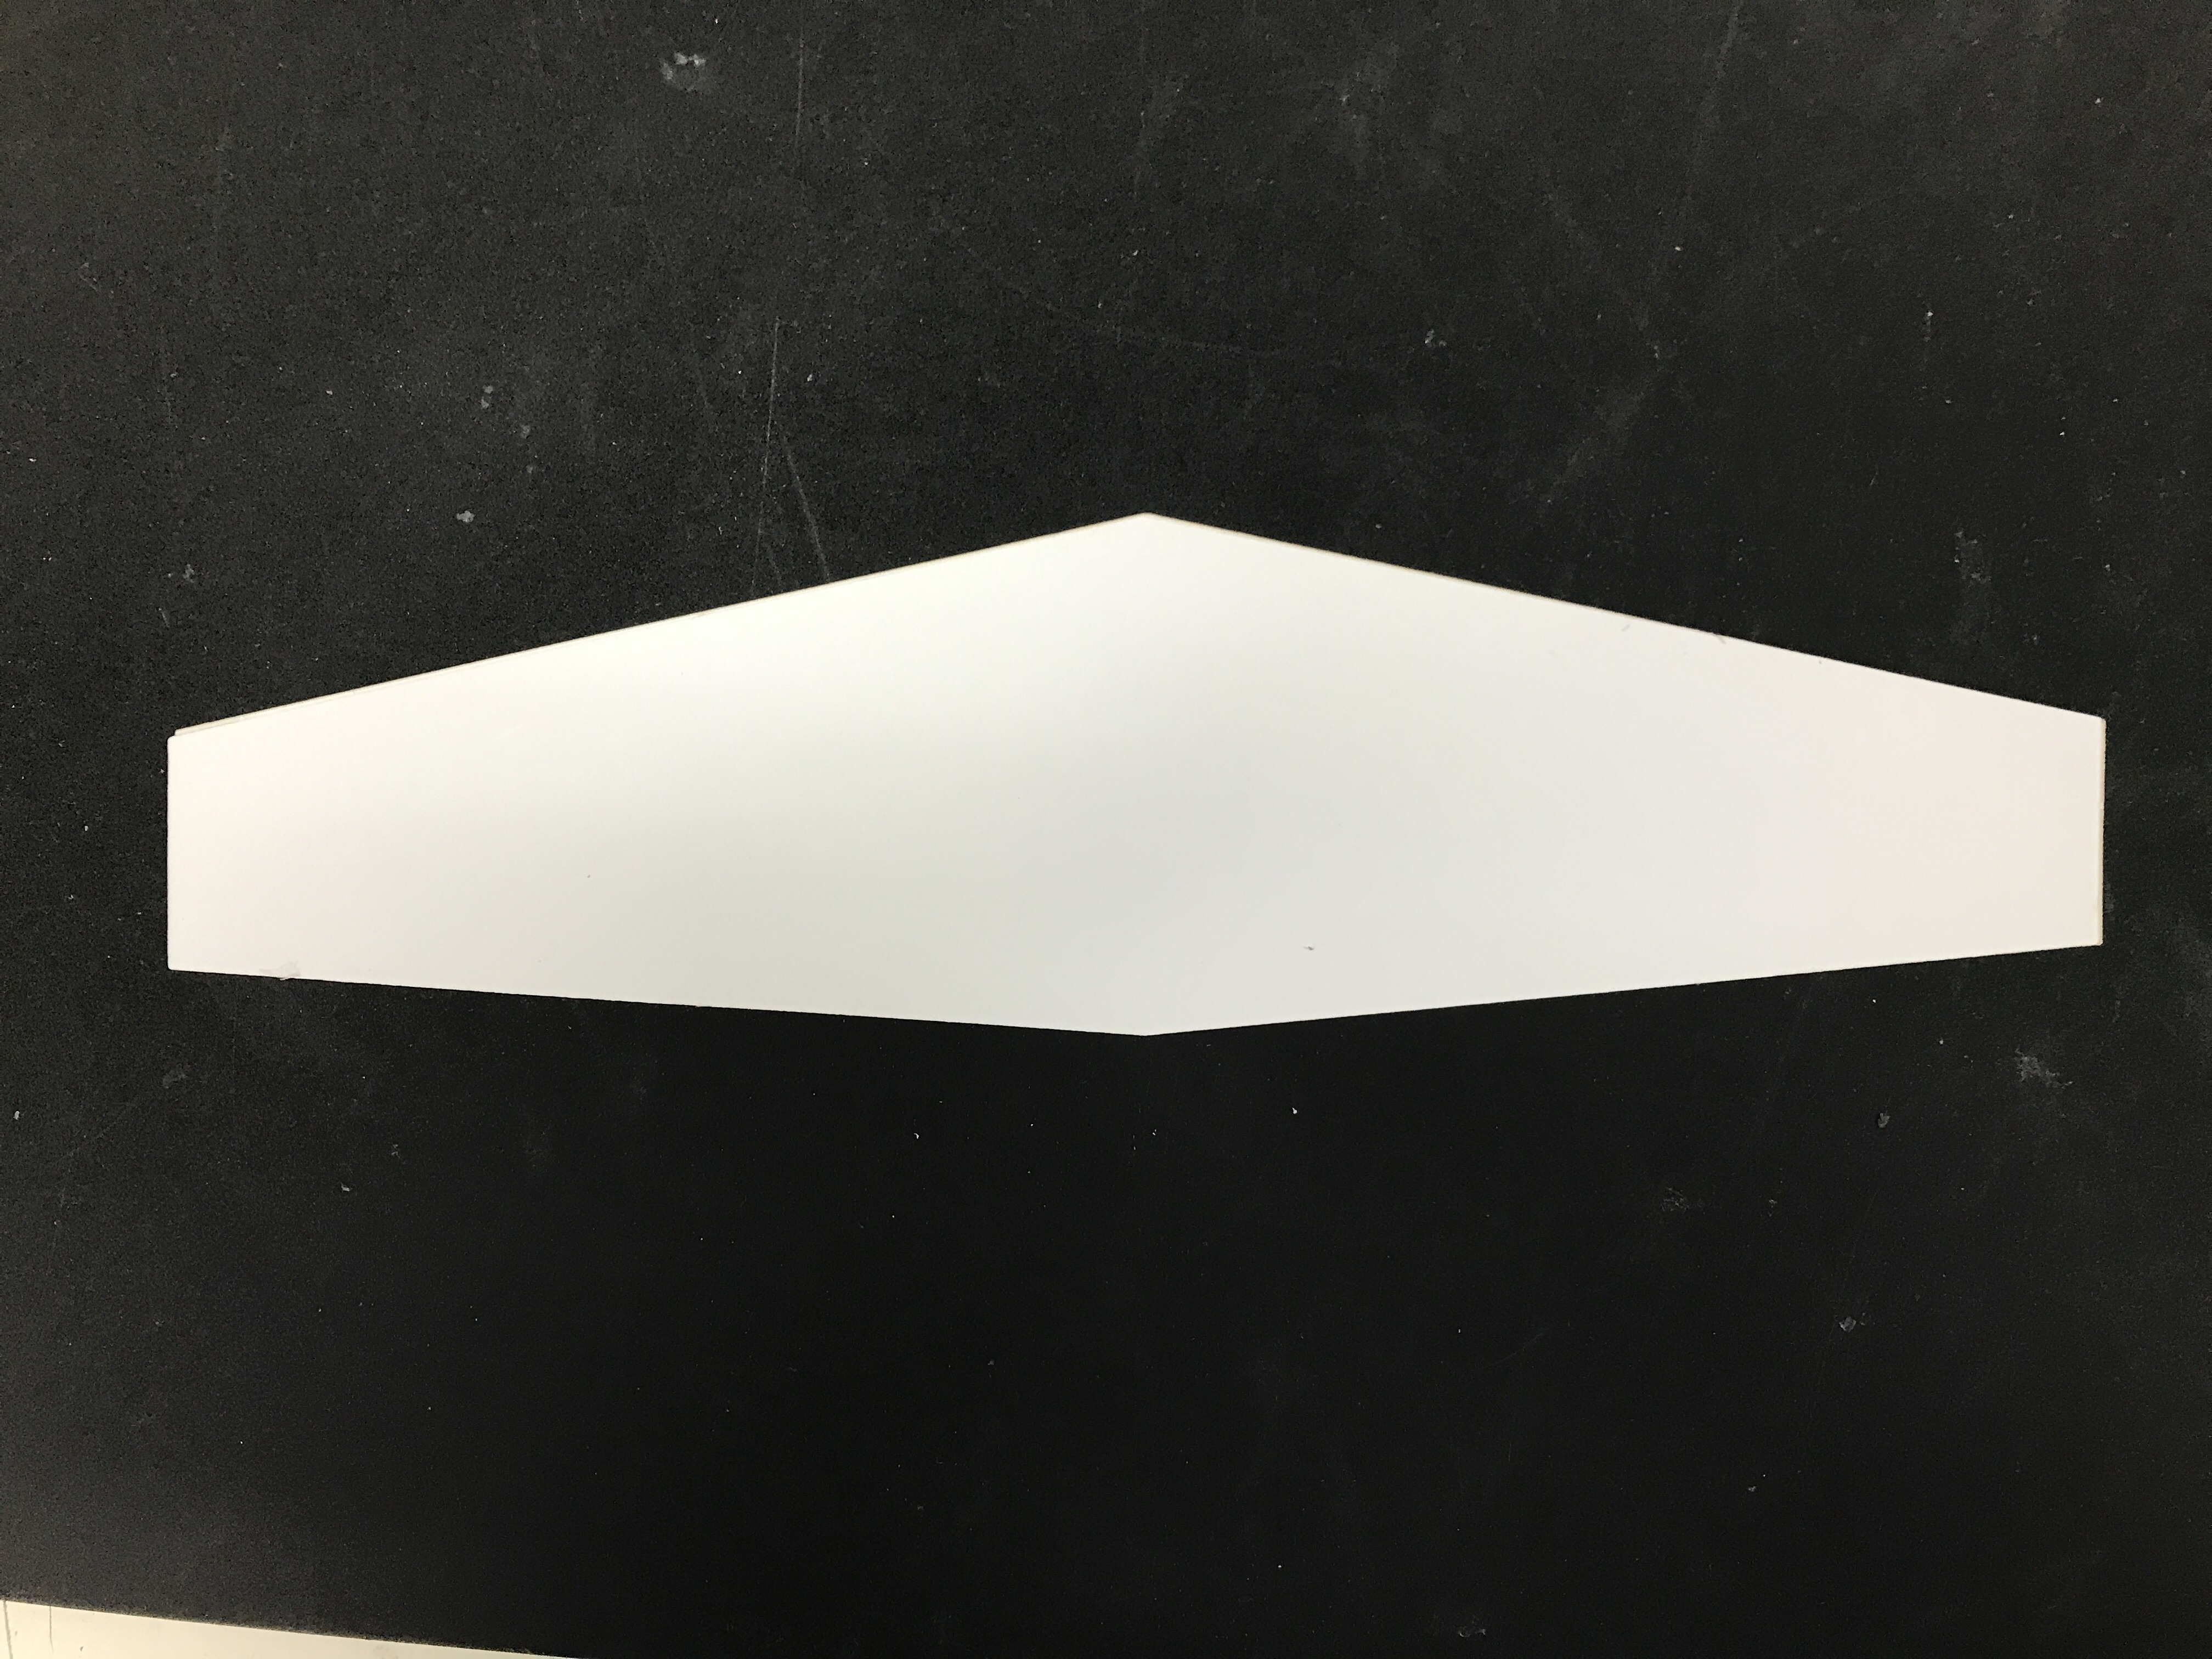
\includegraphics[width=140mm]{OK.JPG}
    \end{center}
  \caption{綺麗なつばさ}
 \label{fig:OK}
\end{figure}

\begin{figure}[htbp]
  \begin{center}
    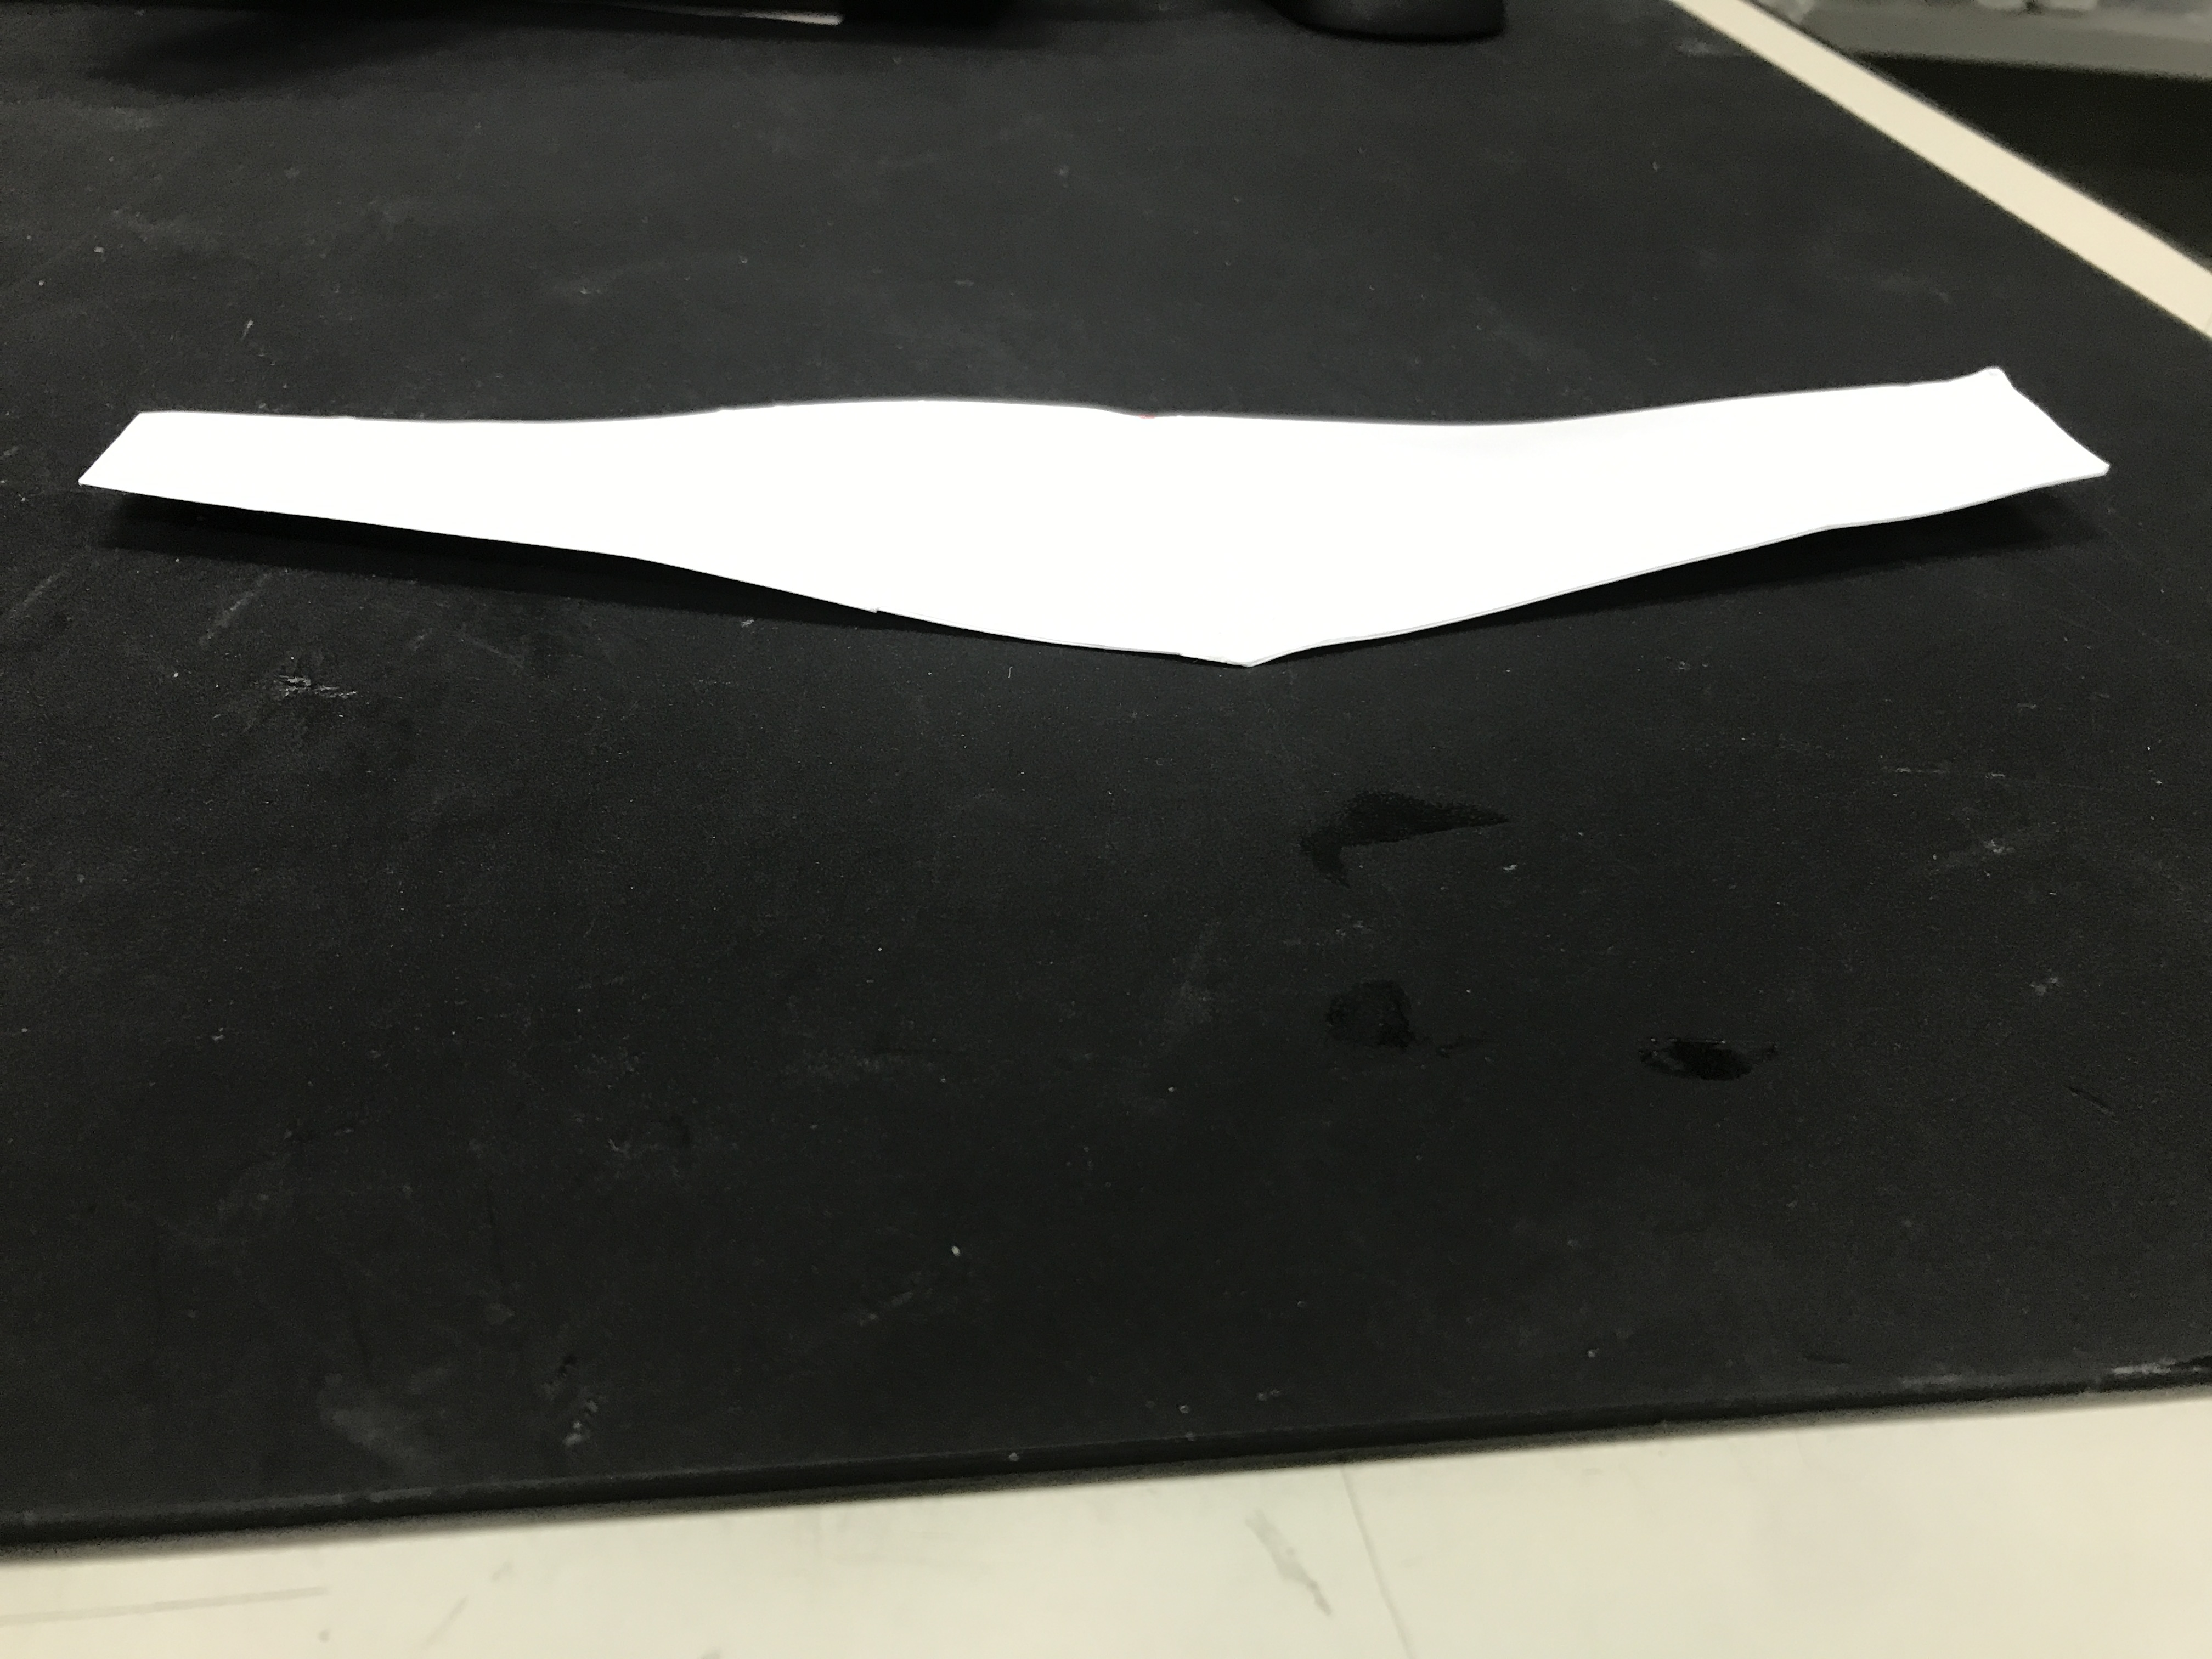
\includegraphics[width=140mm]{NG.JPG}
    \end{center}
  \caption{凸凹な翼}
 \label{fig:NG}
\end{figure}

\section{組み立て}
上記の方法で加工や接着を行った後組み立てを行う.翼をストローに張り付ける際,翼が傾かないようにしないといざ飛ばす時左に旋回したり右に旋回してしまうので注意が必要である.また水平に取り付けを行った場合でも左右に旋回する事がある.原因としては確認できない細かなズレのため生じている.そのため旋回したほうの主翼のエルロンを調整を行い旋回を修正していく必要がある.飛行機の各名称の図を図\ref{fig:er}に示す.
垂直尾翼に関しては尾翼と設置する面積が少ないため接着に安定感がなくすぐ折れてしまう.したがって図のようにテープを貼るなどして折れてしまわない工夫を行わないといけない.

\begin{figure}[htbp]
  \begin{center}
    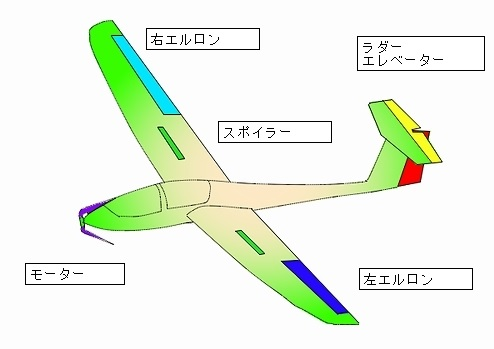
\includegraphics[width=140mm]{er.JPG}
    \end{center}
  \caption{飛行機の各名称}
 \label{fig:er}
\end{figure}